
\chapter{OWASP Top Ten
}\label{kap:owasptopten}

This section describes how prepared are we against common threats listed in OWASP Top 10 //TODO

%TODO SORT ME prob A1-10

\section{Injection}

Injection attack happens when web application receives input which can be interpreted a command or query. One of the most notable injection attacks is SQL injection, which can lead to reading, modifying or deleting database by an attacker. Typically injection attacks happens through form input fields, like those in login form.

To avoid this, user input must be validated before it is sent as a query. In addition we also use SQLAlchemy which automatically quotes special characters like apostrophes in data.

(ref. http://www.rmunn.com/sqlalchemy-tutorial/tutorial.html) % TODO
% TODO rest to be finished by lukas

\section{A07:2021 Identification and Authentication Failures}

This security fault is known as Broken Authentication, which is about user´s identity is breached with weaknesses with the authentication in our application, for example using automated attacks. We have implemented a few things to mitigate this, as reCAPTCHA, ratelimit , two factor authentication, strong password etc.   

Firstly to avoid brute forcing and automated attacks, reCAPTCHA and ratelimit has a huge impact on this. The way we implanted this is making a reCAPTCHA user on google and verifying this in our flask WTforms. <code> reCAPTCHA = recaptchaField() <code>. It is possible to bypass wtforms validators/reCAPTCHA so we also made a request limiter, which makes a response and blocks out the user, which will reset in a couple of minutes. We have sat the limit to 60 POST/GET request since that should be more than enough for a normal user. Anything more than that we will block it. The code we used to implement this is:

\begin{python}
@auth.app_errorhandler(429)
def ratelimit_handler(e):
    try:
        message = "Request Limit: User: " + current_user.username\
                  + ". Time: " + str(datetime.datetime.now())
    except:
        message = "Request Limit: User: None . Time: "\
                  + str(datetime.datetime.now())
    db.session.add(Logs(log=message))
    db.session.commit()
    logout_user()
    session['logged_in'] = False
    return make_response(
        jsonify(
            error="Ratelimit exceeded %s" % e.description + 
                  ". Our BOT killer detected unusual many request."+
                  "Please slow down or turn of your BOT!")
        , 429
    )
\end{python}

If an attacker manages to get ahold of an users password we uses two factor authentication which is compatible with google authenticator. We uses this verification after each transaction, deposit and when we log-in. This makes the attacker not being able to access that users account without also having access to their google authenticator app. This acts like a second layer to the users security.  The code we used to implement this is <code>
We have also implemented many more features to prevent this type of security breach like same message if failed log in attempt but we won´t cover this since it is not the most important. 

\section{A09 Security Logging and Monitoring Failures}

A09 has been recently more important over the years. This security breach includes not being able to detect or log activity on the website. This includes also securing the log functions so that no malicious attacks can go through this feature. 

In our website we log every major request. This includes log in, sign-up, transactions, ATM deposits and if the user goes over the request limiter and the ratelimit function is called. We log both successes and failures. The way we store the data is in a separate table in the database. We simple store a string of text that is set by the request the user makes. So a typical string will contain the request (log-in/sign-up etc.), username (if exists), failed or passed and then lastly what time it happened. The way we implemented this is: <code>

We also verifies that the input doesn’t contain any illegal character, so the way we log things doesn’t become a security breach, for example injection in to the database. This is because so that it is harder to breach the log and loads of information about users becomes available to the attacker. The code for this check is: 

\begin{python}
def validate_username(username):
    """Checks for valid username (only letters and numbers)"""
    if len(username) < 2 or len(username) > 50:
        flash("Username must be longer than one character,"+
              "and shorter than fifty", category='error')
        return False

    # If only contains small and big letters, and numbers
    if re.search("^[a-zA-Z0-9s]+$", username):
        return True
    flash("Username can only contain letters and numbers",
        category='error')
    return False
\end{python}

Another logging information we have is ReCAPTCHA. As you can see from picture below is that we can see the statistic of the uses of it and if it have detected any unusual activity. It will also send us an email if detected anything unusual. The negativity with this is that reCAPTCHA uses a long time to update. It uses a couple of days usually, therefore we cannot solely trust on this. 

\begin{figure}[H]
    \centering
    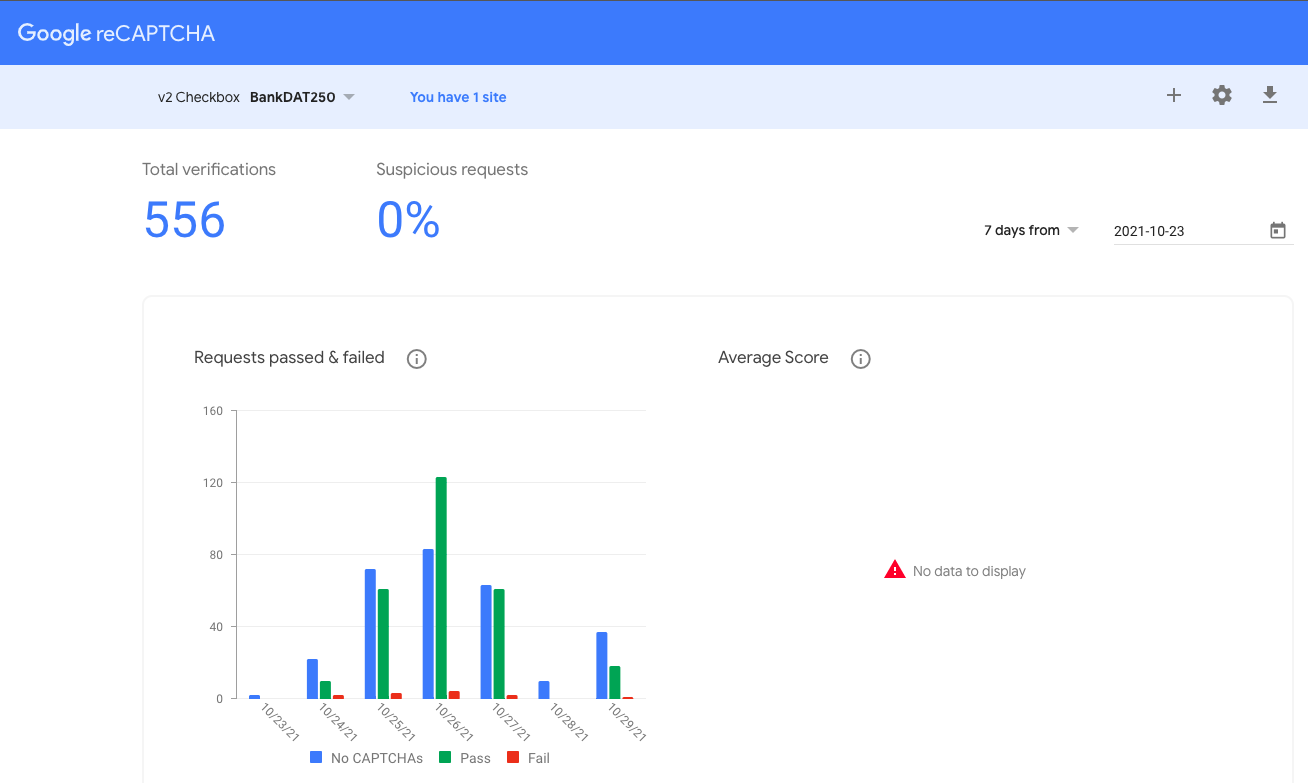
\includegraphics[width=\textwidth]{pics/recaptchaLog.png}
    \caption{reCAPTCHA Log}
    \label{fig:cha3fig1recaptchalog}
 \end{figure}

\section{A05 Security Misconfiguration}

This security flaw is about misconfiguration of the website, for example available administrative interfaces, not good error handling and still being in debug mode etc.
For example when we are in development face we often use debug mode, which makes it easier to debug error in the website but also it automatically update your code changes (at least in flask). This can be harmful if not reverted back on deployment. This is because an attacker loves to get error messages and can easily understand how your website is flawed and in which way.  This is simply to remember to disable debug mode which is this line of code: <code>
Another thing we need to is have an error handler for flask, so that the attacker won´t really know what error happened if it manages to create one. In our application we simply check for any errors and if detected we flash a red error message and redirects you do the home page. This also acts as a protective layer against crashing the website. The code used is:

\begin{python}
@auth.errorhandler(Exception)
def basic_error(e):
    """Error handler so flashes message
    and redirects user if error occur"""
    flash("Something went wrong", category='error')
    return redirect(url_for('auth.home_login'))
\end{python}

Since we don´t use any administrative access because of the potential of being a security risk, all the admin access must have access to the deployment website and can make changes there, not directly on the website. Therefore all users have the same access when using the website.

\section{A04 Insecure Design}

This new category in OWASP Top 10 is about flaws in design and system architecture. Some weaknesses and technical requirements need to be thought about before starting the implementation. An example of that could be risk profiling and resource management. “A house is as strong as its foundation”. 
While creating this application we have researched secure way to design systems and created threat model to help us recognize and evaluate possible vulnerabilities. We have also prepared for some known attack methods and evaluated which external packages will be used based on security. Furthermore everything that has been implemented we focus on security, for example by setting bounds to user input so that it don’t cause buffer overflow, sanitize all inputs of a user and a robust error handler so it doesn’t crash our website. 

\section{A06 Vulnerable and Outdated Components}

This Owasp category is about use of unmaintained or out-of-date components with known vulnerabilities. It may become hard to track all dependencies together with nested dependencies.
To work against this we remove all unused dependencies and we check those which are being used, so we would know when one becomes unmaintained. All dependencies are kept on a list together with version used so the process becomes semi-automated.

\section{A01 Broken Access Control}

The number one of security breaches is Broken Access Control and therefore very important for our development team. This breach is about being able to acts outside of their intendent permissions. For example if a user is not logged in it can’t view pages on the website that they are not authorized to see or make requests. 

A way to mitigate this flaw is by using flask-login. When a user login we use the login(user) code. This logs the user inn and can access routes in our website that requires a user to log-in. We use the “@login required” parameter for the implemented route. The code makes it so that the user that tries to access the page/route must be logged in. When a user logs out we call the code logout(user). This removes the flag that the user is logged in and has now not access to the pages it had when logged in. The code snippets below demonstrate this. 

Lastly to mitigate this security fault is checking if the user has been inactive for more than 5 minutes. This is important if a user forgets to exit the website or logging out, because then the session cookie will still be available. The implementation looks like this:

\begin{python}
@auth.before_request
def before_request():
    """Timeout user when inactive in 5 min"""
    flask.session.permanent = True
    current_app.permanent_session_lifetime\
        = datetime.timedelta(minutes=5)
    flask.session.modified = True
    flask.g.user = flask_login.current_user
\end{python}

\section{A08 Software and Data Integrity Failures}

This new category in 2021 is about making sure application uses trusted packages from external sources. This is because using modules from insecure sources can lead to injection of malicious code into the system.

External packages used in this application are received via python pip to which only maintainers have access to. It shouldn’t be a problem as long as we don’t make a typo in package name – which can be used in “typosquatting” attack, where attacker uploads a malicious code to python pip with a name similar to another package.

We can also manually verify that it was produced by the publisher by downloading package and checking signature file.